\begin{frame}
	\frametitle{Fondements}
	\begin{itemize}
		\item Utilisable en ligne
		\item Ensemble de la chaîne de production
		\item Accessible : langage ouvert basé sur XML
	\end{itemize}
	\begin{figure}
		\centering
		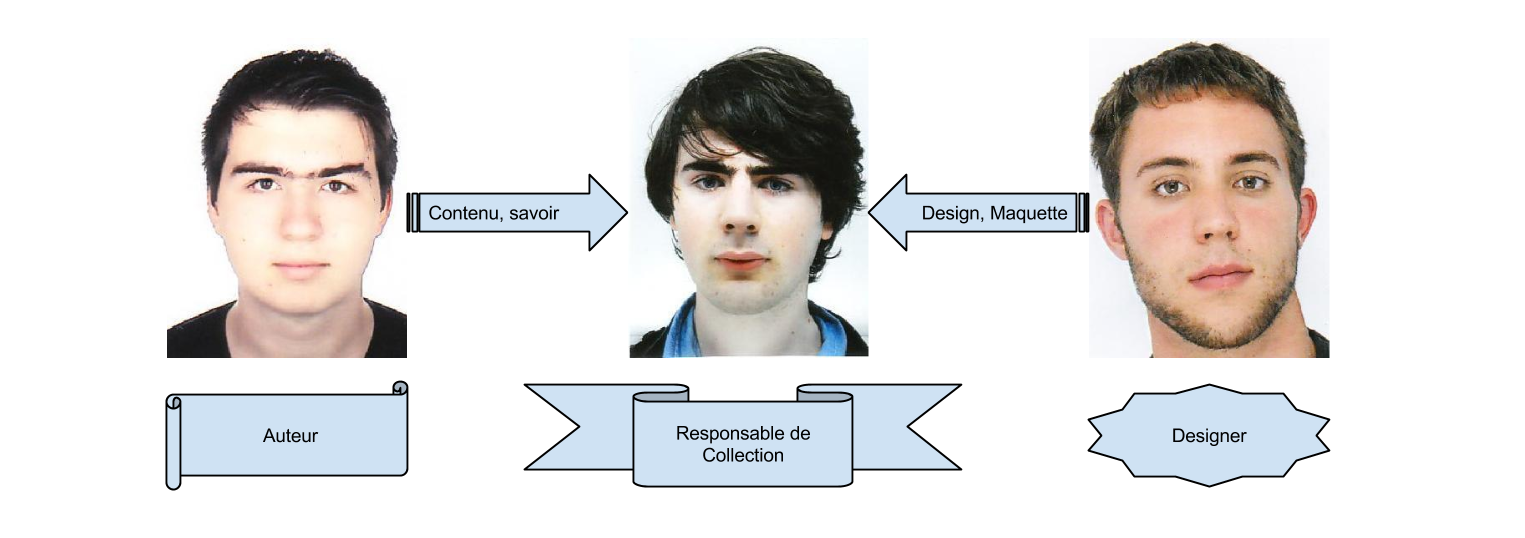
\includegraphics[scale=0.2]{resources/lesBGdeLaDOC.png}
	\end{figure}
\end{frame}

\begin{frame}
	\frametitle{Production basée sur XSL-T}
	\begin{itemize}
		\item source : matière pédagogique -> cible : document
		\item Cible doit toujours avoir la même forme
	\end{itemize}
	\begin{block}{Interactions}
	\begin{itemize}
		\item Responsable \& auteur : concepts -> balises
		\item Responsable \& graphiste : maquette -> action des balises
	\end{itemize}	
	\end{block}

\end{frame}

\begin{frame}
	\frametitle{Exemple : toxicité}
	\begin{itemize}
		\item Problématique pédagogique : toxicité
		\item Problématique de médiatisation : illustrer le concept
	\end{itemize}
	\begin{block}{Définition d'une balise}
			\texttt{\$tox chlore}
	\end{block}
	\begin{itemize}
		\item Page web : popup
		\item Document : cadre de rappel
		\item Puissance : séparation forme / contenu
	\end{itemize}

\end{frame}